\documentclass[a4paper,12pt,twoside]{report}
\usepackage[left=2cm,right=2cm,top=2cm,bottom=3cm]{geometry}
\usepackage[spanish]{babel}
\usepackage[utf8]{inputenc}
\usepackage{svg}
\usepackage{xcolor}
\usepackage{graphicx}
\usepackage{listingsutf8}
\usepackage{apalike}
\lstset{literate={ñ}{{\~n}}1}
\usepackage{float}
\usepackage{tipa}
\usepackage{lscape} 



\usepackage{xcolor}
\usepackage{soul}
\newcommand{\macb}{\textcolor{red}}

\graphicspath{ {./imagenes/} }

\usepackage{graphicx}
\usepackage{verbatim}
\usepackage{latexsym}
\usepackage{mathchars}
\usepackage{setspace}
\usepackage{tikz}
\usepackage{booktabs}
\usepackage{rotating}
\usepackage{tabularx}
\usepackage{lscape} 
\usepackage{tipa}
\usepackage{float}
\usepackage{url}
% \usepackage{apacite}
\usetikzlibrary{positioning}

\setlength{\parskip}{\medskipamount}  % a little space before a \par
\setlength{\parindent}{0pt}	      % don't indent first lines of paragraphs
%UHEAD.STY  If this is included after \documentstyle{report}, it adds
% an underlined heading style to the LaTeX report style.
% \pagestyle{uheadings} will put underlined headings at the top
% of each page. The right page headings are the Chapter titles and
% the left page titles are supplied by \def\lefthead{text}.

% Ted Shapin, Dec. 17, 1986

\makeatletter
\def\chapapp2{Chapter}

\def\appendix{\par
 \setcounter{chapter}{0}
 \setcounter{section}{0}
 \def\chapapp2{Appendix}
 \def\@chapapp{Appendix}
 \def\thechapter{\Alph{chapter}}}

\def\ps@uheadings{\let\@mkboth\markboth
% modifications
\def\@oddhead{\protect\underline{\protect\makebox[\textwidth][l]
		{\sl\rightmark\hfill\rm\thepage}}}
\def\@oddfoot{}
\def\@evenfoot{}
\def\@evenhead{\protect\underline{\protect\makebox[\textwidth][l]
		{\rm\thepage\hfill\sl\leftmark}}}
% end of modifications
\def\chaptermark##1{\markboth {\ifnum \c@secnumdepth >\m@ne
 \chapapp2\ \thechapter. \ \fi ##1}{}}%
\def\sectionmark##1{\markright {\ifnum \c@secnumdepth >\z@
   \thesection. \ \fi ##1}}}
\makeatother
%%From: marcel@cs.caltech.edu (Marcel van der Goot)
%%Newsgroups: comp.text.tex
%%Subject: illegal modification of boxit.sty
%%Date: 28 Feb 92 01:10:02 GMT
%%Organization: California Institute of Technology (CS dept)
%%Nntp-Posting-Host: andromeda.cs.caltech.edu
%%
%%
%%Quite some time ago I posted a file boxit.sty; maybe it made it
%%to some archives, although I don't recall submitting it. It defines
%%	\begin{boxit}
%%	...
%%	\end{boxit}
%%to draw a box around `...', where the `...' can contain other
%%environments (e.g., a verbatim environment). Unfortunately, it had
%%a problem: it did not work if you used it in paragraph mode, i.e., it
%%only worked if there was an empty line in front of \begin{boxit}.
%%Luckily, that is easily corrected.
%%
%%HOWEVER, apparently someone noticed the problem, tried to correct it,
%%and then distributed this modified version. That would be fine with me,
%%except that:
%%1. There was no note in the file about this modification, it only has my
%%   name in it.
%%2. The modification is wrong: now it only works if there is *no* empty
%%   line in front of \begin{boxit}. In my opinion this bug is worse than
%%   the original one.
%%
%%In particular, the author of this modification tried to force an empty
%%line by inserting a `\\' in the definition of \Beginboxit. If you have
%%a version of boxit.sty with a `\\', please delete it. If you have my
%%old version of boxit.sty, please also delete it. Below is an improved
%%version.
%%
%%Thanks to Joe Armstrong for drawing my attention to the bug and to the
%%illegal version.
%%
%%                                          Marcel van der Goot
%% .---------------------------------------------------------------
%% | Blauw de viooltjes,                    marcel@cs.caltech.edu
%% |    Rood zijn de rozen;
%% | Een rijm kan gezet
%% |    Met plaksel en dozen.
%% |


% boxit.sty
% version: 27 Feb 1992
%
% Defines a boxit environment, which draws lines around its contents.
% Usage:
%   \begin{boxit}
%	... (text you want to be boxed, can contain other environments)
%   \end{boxit}
%
% The width of the box is the width of the contents.
% The boxit* environment behaves the same, except that the box will be
% at least as wide as a normal paragraph.
%
% The reason for writing it this way (rather than with the \boxit#1 macro
% from the TeXbook), is that now you can box verbatim text, as in
%   \begin{boxit}
%   \begin{verbatim}
%   this better come out in boxed verbatim mode ...
%   \end{verbatim}
%   \end{boxit}
%
%						Marcel van der Goot
%						marcel@cs.caltech.edu
%

\def\Beginboxit
   {\par
    \vbox\bgroup
	   \hrule
	   \hbox\bgroup
		  \vrule \kern1.2pt %
		  \vbox\bgroup\kern1.2pt
   }

\def\Endboxit{%
			      \kern1.2pt
		       \egroup
		  \kern1.2pt\vrule
		\egroup
	   \hrule
	 \egroup
   }	

\newenvironment{boxit}{\Beginboxit}{\Endboxit}
\newenvironment{boxit*}{\Beginboxit\hbox to\hsize{}}{\Endboxit}
\pagestyle{empty}

\setlength{\parskip}{2ex plus 0.5ex minus 0.2ex}
\setlength{\parindent}{0pt}

\makeatletter  %to avoid error messages generated by "\@". Makes Latex treat "@" like a letter

\linespread{1.5}
\def\submitdate#1{\gdef\@submitdate{#1}}

\def\maketitle{
  \begin{titlepage}{
    %\linespread{1.5}
    \Large Universidad del Valle 
    \linebreak
    Facultad de Ingeniería
    \linebreak
    Escuela de Ingeniería de Sistemas y Computación 
    
    \rm
    \vskip 3in
    \Large \bf \@title \par
  }
  \vskip 0.3in
  \par
  {\Large \@author}
  
  
  {\Large 201802679}
  \linebreak
  {\large mauricio.collazos@correounivalle.edu.co}
  \vskip 1in
  {\large Dirigido por}
  \linebreak
  {\large Raúl Ernesto Gutierrez de Piñeres Reyes Ph.D.}
  \linebreak
  {\large Co-dirigido por}
  \linebreak
  {\large Maria Andrea Cruz Blandón M.Sc.}
  \vskip 2in
  \par
  \linebreak
  Maestría en Ingeniería con énfasis en Ingeniería de Sistemas y Computación
  \linebreak
  2021
  \vfil
  
  \end{titlepage}
}

\def\titlepage{
  \newpage
  \centering
  \linespread{1}
  \normalsize
  \vbox to \vsize\bgroup\vbox to 9in\bgroup
}
\def\endtitlepage{
  \par
  \kern 0pt
  \egroup
  \vss
  \egroup
  \clearpage
}

\def\abstract{
  \begin{center}{
    \large\bf Resumen}
  \end{center}
  \small
  %\def\baselinestretch{1.5}
  \linespread{1.5}
  \normalsize
}

\def\endabstract{
  \par
}

\newenvironment{acknowledgements}{
  \cleardoublepage
  \begin{center}{
    \large \bf Acknowledgements}
  \end{center}
  \small
  \linespread{1.5}
  \normalsize
}{\cleardoublepage}
\def\endacknowledgements{
  \par
}

\newenvironment{dedication}{
  \cleardoublepage
  \begin{center}{
    \large \bf Dedication}
  \end{center}
  \small
  \linespread{1.5}
  \normalsize
}{\cleardoublepage}
\def\enddedication{
  \par
}

\def\preface{
    \pagenumbering{roman}
    \pagestyle{plain}
    \doublespacing
}

\def\body{
    \clearpage
    \pagestyle{uheadings}
    \tableofcontents
    \pagestyle{plain}
    \clearpage
    \pagestyle{uheadings}
    \listoftables
    \pagestyle{plain}
    \clearpage
    \pagestyle{uheadings}
    \listoffigures
    \pagestyle{plain}
    \clearpage
    \pagestyle{uheadings}
    \pagenumbering{arabic}
    \doublespacing
}

\makeatother  %to avoid error messages generated by "\@". Makes Latex treat "@" like a letter

\newcommand{\ipc}{{\sf ipc}}

\newcommand{\Prob}{\bbbp}
\newcommand{\Real}{\bbbr}
\newcommand{\real}{\Real}
\newcommand{\Int}{\bbbz}
\newcommand{\Nat}{\bbbn}

\newcommand{\NN}{{\sf I\kern-0.14emN}}   % Natural numbers
\newcommand{\ZZ}{{\sf Z\kern-0.45emZ}}   % Integers
\newcommand{\QQQ}{{\sf C\kern-0.48emQ}}   % Rational numbers
\newcommand{\RR}{{\sf I\kern-0.14emR}}   % Real numbers
\newcommand{\KK}{{\cal K}}
\newcommand{\OO}{{\cal O}}
\newcommand{\AAA}{{\bf A}}
\newcommand{\HH}{{\bf H}}
\newcommand{\II}{{\bf I}}
\newcommand{\LL}{{\bf L}}
\newcommand{\PP}{{\bf P}}
\newcommand{\PPprime}{{\bf P'}}
\newcommand{\QQ}{{\bf Q}}
\newcommand{\UU}{{\bf U}}
\newcommand{\UUprime}{{\bf U'}}
\newcommand{\zzero}{{\bf 0}}
\newcommand{\ppi}{\mbox{\boldmath $\pi$}}
\newcommand{\aalph}{\mbox{\boldmath $\alpha$}}
\newcommand{\bb}{{\bf b}}
\newcommand{\ee}{{\bf e}}
\newcommand{\mmu}{\mbox{\boldmath $\mu$}}
\newcommand{\vv}{{\bf v}}
\newcommand{\xx}{{\bf x}}
\newcommand{\yy}{{\bf y}}
\newcommand{\zz}{{\bf z}}
\newcommand{\oomeg}{\mbox{\boldmath $\omega$}}
\newcommand{\res}{{\bf res}}
\newcommand{\cchi}{{\mbox{\raisebox{.4ex}{$\chi$}}}}
%\newcommand{\cchi}{{\cal X}}
%\newcommand{\cchi}{\mbox{\Large $\chi$}}

% Logical operators and symbols
\newcommand{\imply}{\Rightarrow}
\newcommand{\bimply}{\Leftrightarrow}
\newcommand{\union}{\cup}
\newcommand{\intersect}{\cap}
\newcommand{\boolor}{\vee}
\newcommand{\booland}{\wedge}
\newcommand{\boolimply}{\imply}
\newcommand{\boolbimply}{\bimply}
\newcommand{\boolnot}{\neg}
\newcommand{\boolsat}{\!\models}
\newcommand{\boolnsat}{\!\not\models}


\newcommand{\op}[1]{\mathrm{#1}}
% \newcommand{\s}[1]{\ensuremath{\mathcal #1}}

% Properly styled differentiation and integration operators
\newcommand{\diff}[1]{\mathrm{\frac{d}{d\mathit{#1}}}}
\newcommand{\diffII}[1]{\mathrm{\frac{d^2}{d\mathit{#1}^2}}}
\newcommand{\intg}[4]{\int_{#3}^{#4} #1 \, \mathrm{d}#2}
\newcommand{\intgd}[4]{\int\!\!\!\!\int_{#4} #1 \, \mathrm{d}#2 \, \mathrm{d}#3}

% Large () brackets on different lines of an eqnarray environment
\newcommand{\Leftbrace}[1]{\left(\raisebox{0mm}[#1][#1]{}\right.}
\newcommand{\Rightbrace}[1]{\left.\raisebox{0mm}[#1][#1]{}\right)}

% Funky symobols for footnotes
\newcommand{\symbolfootnote}{\renewcommand{\thefootnote}{\fnsymbol{footnote}}}
% now add \symbolfootnote to the beginning of the document...

\newcommand{\normallinespacing}{\renewcommand{\baselinestretch}{1.5} \normalsize}
\newcommand{\mediumlinespacing}{\renewcommand{\baselinestretch}{1.2} \normalsize}
\newcommand{\narrowlinespacing}{\renewcommand{\baselinestretch}{1.0} \normalsize}
\newcommand{\bump}{\noalign{\vspace*{\doublerulesep}}}
\newcommand{\cell}{\multicolumn{1}{}{}}
\newcommand{\spann}{\mbox{span}}
\newcommand{\diagg}{\mbox{diag}}
\newcommand{\modd}{\mbox{mod}}
\newcommand{\minn}{\mbox{min}}
\newcommand{\andd}{\mbox{and}}
\newcommand{\forr}{\mbox{for}}
\newcommand{\EE}{\mbox{E}}

\newcommand{\deff}{\stackrel{\mathrm{def}}{=}}
\newcommand{\syncc}{~\stackrel{\textstyle \rhd\kern-0.57em\lhd}{\scriptstyle L}~}

\def\coop{\mbox{\large $\rhd\!\!\!\lhd$}}
\newcommand{\sync}[1]{\raisebox{-1.0ex}{$\;\stackrel{\coop}{\scriptscriptstyle
#1}\,$}}

\newtheorem{definition}{Definition}[chapter]
\newtheorem{theorem}{Theorem}[chapter]

\newcommand{\Figref}[1]{Figure~\ref{#1}}
\newcommand{\fig}[3]{
 \begin{figure}[!ht]
 \begin{center}
 \scalebox{#3}{\includegraphics{figs/#1.ps}}
 \vspace{-0.1in}
 \caption[ ]{\label{#1} #2}
 \end{center}
 \end{figure}
}

\newcommand{\figtwo}[8]{
 \begin{figure}
 \parbox[b]{#4 \textwidth}{
 \begin{center}
 \scalebox{#3}{\includegraphics{figs/#1.ps}}
 \vspace{-0.1in}
 \caption{\label{#1}#2}
 \end{center}
 }
 \hfill
 \parbox[b]{#8 \textwidth}{
 \begin{center}
 \scalebox{#7}{\includegraphics{figs/#5.ps}}
 \vspace{-0.1in}
 \caption{\label{#5}#6}
 \end{center}
 }
 \end{figure}
}

\title{Anotación automática de un corpus hablado de licencia abierta y larga duración para el lenguaje Español}
\author{Mauricio Collazos}
\date{March 2021}

\begin{document}

\maketitle

\begin{abstract}
    Los recursos abiertos para el procesamiento, reconocimiento, generación y demás tareas relacionadas con las tecnologías del lenguaje hablado son parte fundamental del proceso académico e investigativo. Estos recursos deben contener características muy específicas para la ejecución adecuada de la tarea relacionada, donde los niveles de anotación, duración de las grabaciones, variedad de locutores, balance de género, tamaño del vocabulario, relación de señal/ruido y conjunto de datos para pruebas son fundamentales. A pesar de existir diversos recursos disponibles para realizar las tareas mencionadas, los recursos abiertos para trabajar las tecnologías del habla en la lengua española son escasos y en muchos casos insuficientes para realizar comparaciones con investigaciones del estado del arte propuestas para otros lenguajes. Este trabajo realiza una exploración de los recursos abiertos para el español y propone mecanismos para segmentar audio libros publicados por voluntarios bajo licencias abiertas en recursos apropiados para el procesamiento de voz.
\end{abstract}
\chapter*{Agradecimientos}

Tengo que darle mil gracias a Maria Andrea Cruz Blandón por todas esas horas dedicadas a conversar, guiar y estructurar este trabajo, sin su ayuda sin duda este no se habría podido llevar a cabo.

De igual manera al profesor Raul Gutierrez de Piñeres Ph.D quien ha estado al pendiente de todo el proceso y a la Universidad del Valle por brindarme las herramientas y recursos necesarios para realizar esta investigación.

También a mi familia y amigos, cuyo animo fue de vital importancia.
\body

\chapter{Introducción}

El procesamiento de voz es un área de investigación activa que combina aspectos del procesamiento de señales y estudio del lenguaje natural. Entre las tareas destacadas de esta área de investigación destacan la síntesis y el reconocimiento de voz, que han sido un problema abordado desde hace más de un siglo, con aproximaciones diversas que van desde el procesamiento de señales hasta las redes neuronales profundas.  En las últimas décadas de investigación en este campo se han logrado mejores resultados en diversas tareas como la síntesis de voz haciendo uso de gran volumen de datos.

Los corpus o colección de datos deben cumplir con características para poder ser usados en investigación, entre las que se encuentran género, dialecto y edad del locutor, las condiciones de grabación, ruido de ambiente, origen de la grabación, el lenguaje usado, y el tipo de distribución.

La creación de corpus para abordar las distintas tareas en el procesamiento de voz es por lo general costosa, pues incluye la consecución de locutores, los recursos de hardware para realizar las grabaciones en condiciones apropiadas y el personal para el enriquecimiento de los recursos, como la segmentación, anotación y clasificación. Dado que este proceso es costoso, muchos recursos se distribuyen bajo licencias cerradas, lo que dificulta el acceso de los mismos.

Este trabajo busca la creación de un corpus usando grabaciones previamente recolectadas y distribuidas bajo licencia abierta, utilizando mecanismos automáticos para la segmentación y anotación de los mismos.

\section{Definición del problema}

Los recursos para la investigación de tecnologías del habla son de vital importancia para la generación y validación de nuevo conocimiento en el área. En la actualidad donde la investigación se ha decantado en su mayoría por el aprendizaje de máquina utilizando mecanismos de aprendizaje supervisado, semi supervisado y no supervisado \cite{Chiu2018} \cite{AmazonSemiSupervised}  \cite{ZeroResources}, la calidad y tamaño de los corpus usados para el entrenamiento, validación y pruebas definen en gran medida los resultados de la investigación \cite{Hernandez-Mena2017AutomaticResources}.


Como la creación de corpus es costosa \cite{googleTTSLatinAmericanSpanishCorpus}, se propone utilizar grabaciones distribuidas bajo licencia libre y realizar el procesamiento requerido para formar un corpus para el procesamiento de voz.

Se usarán las grabaciones del proyecto Librivox \cite{LibriVox}, una iniciativa que, por medio de voluntarios, graba audio libros que pertenecen al dominio público. En su mayoría, los audio libros se encuentran publicados en el proyecto Gutenberg \cite{gutenberg}. Cada libro es grabado por capítulo y cada capítulo es grabado por un solo locutor.

Dado que las grabaciones tienen una longitud de varios minutos, se realizará un proceso de segmentación donde a partir de cada grabación se obtienen trozos mas pequeños de tamaño conforme a otros corpus. Posteriormente se realizará un proceso de alineación sobre estos segmentos, donde se determinará a partir de la información acústica de cada segmento de grabación, la declaración correspondiente.


\section{Justificación}

En la literatura se encuentran recursos representativos reconocidos para realizar tareas comunes como el reconocimiento automático del habla y la síntesis del habla como, TIMIT \cite{PriceTheRecognition}, Darpa Resource Management \cite{Lucke1992ExpandingCorpus}, Switchboard \cite{Godfrey1992SWITCHBOARD:Development}, Call Home  \cite{Fu-HuaLiuSpeechCorpus},  Cambridge Read News \cite{RobinsonWSJCAM0:RECOGNITION}, Aurora Digits \cite{EvansEfficientCorpus}, Fisher \cite{CieriTheSpeech-to-Text} y Libri Speech \cite{LIBRISPEECH}. Estos corpus se anotados a varios niveles, desde el nivel fonético, donde se describe los momentos en el tiempo donde inicia y termina un fonema; hasta el nivel de declaración donde s\'olo se relaciona una frase típicamente corta con su correspondiente grabación. Todos estos recursos son de lengua inglesa. En la tabla \ref{tab:english_corpora} se extendiende la información de estos recursos en inglés.

\begin{table}[H]
\centering
\caption{Corpus hablados en la lengua inglesa\macb{. La duraci\'on est\'a en horas.}}
% \caption{Speech English Corpus}
\label{tab:english_corpora}
\begin{tabular}{|l|l|l|l|l|}
\textbf{Base de datos} & \textbf{Duración} & \textbf{Vocabulario} & \textbf{Anotación} & \textbf{Licencia}\\
\hline
FISHER\cite{CieriTheSpeech-to-Text}  & más de 2000 & Muy grande &  Declaración & LDC Non-Members\\
\hline
LIBRISPEECH\cite{PanayotovLIBRISPEECH:BOOKS}  & más de 1000 & Muy grande &  Declaración & CC BY 4.0\\
\hline

Switchboard \cite{Godfrey1992SWITCHBOARD:Development}  & 240 & Muy grande & Palabras & LDC Non-Members\\
\hline
\multicolumn{1}{|p{3.4cm}|}{DARPA Resource Management \cite{Lucke1992ExpandingCorpus}} & No especificado  & Grande & Declaración & LDC Non-Members \\
\hline
Cambridge Read News \cite{RobinsonWSJCAM0:RECOGNITION}  & No especificado & Muy grande & Fonético & LDC Non-Members\\
\hline
Call Home  \cite{Fu-HuaLiuSpeechCorpus} & 18.3 & Grande & Declaración & LDC Non-Members\\
\hline
TIMIT \cite{PriceTheRecognition} & 5.4 & Grande & Fonético  & LDC Non-Members\\
\hline
Aurora Digits \cite{EvansEfficientCorpus}  & Menos de 1 & Pequeño & Palabra & ELRA\\
\hline



\end{tabular}
\end{table}

Existen recursos para el español como Call Friend \cite{CALLFRIENDSpa}, Call Home \cite{CALLHOMESpa}, DIMEx100 \cite{Pineda2004DIMEx100:Spanish}, Heróico \cite{heroico}, Voxforfe \cite{Voxforge.org}, Fisher Spanish \cite{FischerSpa}, Albazín \cite{CampilloAlbayzinEvaluation} y CIEMPIESS \cite{Hernandez-MenaCIEMPIESS:Corpus}, los cuales se muestran en la tabla \ref{tab:spanish_corpora}, sin embargo al comparar estos recursos con aquellos en inglés se evidencia una diferencia en duración considerable.

\begin{table}[H]
\centering
\caption{Corpus hablados en la lengua española}
\label{tab:spanish_corpora}
\begin{tabular}{|l|l|l|l|l|}
\textbf{Base de datos} & \textbf{Duración (h)}  & \textbf{Anotación} & Licencia\\
\hline
Fisher Spanish \cite{FischerSpa}  & 163  & Declaración  & LDC Non-Members\\
\hline
CALL FRIEND Spanish \cite{CALLFRIENDSpa}  & 85  & Declaración & LDC Non-Members\\
\hline
CALL HOME Spanish \cite{CALLHOMESpa}  & 70  & Declaración & LDC Non-Members\\
\hline
Voxforge \cite{Voxforge.org}  & 51 & Declaración & GPL\\
\hline
CIEMPIESS\cite{Hernandez-MenaCIEMPIESS:Corpus}  & 17  & Declaración & CC BY-SA 4.0\\
\hline
Heroico \cite{HeroicoCorpus}  & 13 & Declaración & LDC Non-Members  \\
\hline
DIMEx100\cite{Pineda2004DIMEx100:Spanish}  & 5.6  & Fonético & \multicolumn{1}{|p{4cm}|}{Gratis para propósitos académicos}\\
\hline
Albayzín\cite{CampilloAlbayzinEvaluation}  & No especificado  & Declaración & ELRA\\
\hline
\end{tabular}
\end{table}

Se observa en ambas tablas que la mayoría de recursos son de licencia cerrada, sin embargo se destaca el corpus Libri Speech \cite{LIBRISPEECH}, el cual recopila mas de 1000 horas y está distribuido bajo la licencia Creative Commons versión 4. Este corpus se ha convertido en un recurso usado como línea base en múltiples investigaciones \cite{libribox_benchmark1,librilight,libribox_benchmark3}. 

La presencia de este corpus, validada por investigaciones posteriores abre la puerta a desarrollos similares para otros lenguajes utilizando la misma fuente de datos pública Libri Vox. 

% Aunque  existen notables diferencias entre los corpus del español y del inglés, el lenguaje español no se considera un lenguaje con escasos recursos \macb{\st{, pues e}. E}xisten múltiples corpus, bancos de árboles, datos anotados y transcritos, diccionarios y gramáticas formales \cite{CavarGlobalGORILLA}. 

\section{Pregunta de Investigación}



\section{Objetivos}


\subsection{Objetivo general}

Implementar un alineador forzado con el fin de generar automáticamente un corpus para la lengua española de gran vocabulario y larga duración a partir de recursos existentes

\subsection{Objetivos específicos}

\begin{enumerate}
    \item Recolectar recursos hablados existentes y de licencia abierta existentes para la lengua española.
    \item Estudiar los algoritmos para alineadores forzados y sus implementaciones en el estado del arte de forma que soporten la implementación de uno para la lengua española.
    \item Construir un corpus de prueba para medir el desempeño de alineadores forzados en Español.
    \item Implementar un alineador forzado que anote a nivel de palabras un corpus de gran vocabulario y larga duración para la lengua española.
    \item Diseñar de manera empírica un conjunto de pruebas con el fin de establecer el nivel de anotación del alineador

\end{enumerate}
% MACB cambié distribución por estructura y agregué frase de las conclusiones.

\section{Resultados obtenidos}

Se presenta un resumen de los resultados obtenidos en este documento en la tabla
\ref{tab:resultados_obtenidos} donde se relacionan el numeral del objetivo específico, el resultado correspondiente y la sección del documento con la discusión respectiva

\begin{table}[H]
\centering
\caption{Resultados obtenidos}
\label{tab:resultados_obtenidos}
\begin{tabular}{|l|l|l|}
\hline
\multicolumn{1}{|p{2.3cm}|}{\textbf{Objetivo Específico}}  & \textbf{Resultado obtenido}  & \textbf{Capítulo}\\
\hline
1 & Tabla descriptiva con recursos abiertos de voz para el español & 2.1 \\
\hline
2 & Análisis de las técnicas usadas para la construcción de corpus & 2.2 \\
\hline
3 & Anotación manual de un corpus a nivel fonético y de sentencia & 4.1, 4.2 \\
\hline
4 & \multicolumn{1}{|p{12cm}|}{Creación de alineadores forzados basados en estrategias ingénuas y árboles de decisión} & 5.2, 5.3 \\
\hline
5 & \multicolumn{1}{|p{12cm}|}{Extracción de datos de pruebas a partir de corpus anotados manualmente} & 5.4 \\
\hline
\end{tabular}
\end{table}

\section{Estructura del documento}

En el capítulo 2 se muestra una recolección de los recursos existentes y abiertos para el español, realizando un análisis detallado de cada uno de ellos.

En el capítulo 3 se diseñan los recursos de prueba para evaluar el rendimiento del alineador forzado propuesto.

El capítulo 4 muestra múltiples experimentos para los procesos de segmentación y alineación sobre las grabaciones de Libri Vox.

Finalmente, en el capítulo 5 se concluye el proyecto y se discuten posibles trabajos futuros.


\chapter{Revisión de recursos abiertos para el español}

La investigación en tecnologías del habla depende fuertemente en recursos de lenguaje de alta calidad y gran tamaño diseñados para la lengua específica. Los recursos abiertos de este tipo son más escasos en comparación con recursos de pago y la creación de dichos recursos para tareas como reconocimiento y síntesis de voz es costosa, por lo que muchos investigadores optan por crear conjuntos de datos pequeños y enfocados a su investigación.

Para lenguajes diferentes al inglés, la diferencia en disponibilidad de dichos recursos es aún mayor. Este capítulo presenta una compilación de recursos abiertos para tareas relacionados con tecnologías de voz para la lengua española, describiendo cada recurso y proponiendo posibles aplicaciones para cada corpus. Para seleccionar los recursos aquí incluídos se usaron como criterios la visibilidad, disponibilidad y el impacto.

% Veo que todo hace parte de la introducción del capítulo. MACB
% \section{Preámbulo}

Los modelos utilizados regularmente para procesamiento de voz requieren cantidades masivas de datos para lograr buenos resultados. En reconocimiento de voz, sistemas como Listen-Attend-Spell de Google \cite{Chan2016} fue entrenado utilizando 2000 horas aumentadas 20 veces con técnicas de aumento de datos hasta tener un corpus de 40000 horas. Otros modelos del tipo secuencia a secuencia usan 12500 horas de grabación \cite{Chiu2018}. Otros recursos reconocidos en la literatura como  TIMIT \cite{TIMIT} o Swichboard \cite{Switchboard} tienen una duración menor pero su anotación es a nivel fonético o de palabra.

Aunque los esfuerzos para reducir los requerimientos por grandes volúmenes de datos anotados usando aprendizaje semi supervisado \cite{AmazonSemiSupervised} y no supervisado \cite{ZeroResources}, estas aproximaciones requieren una gran cantidad de datos no supervisados.

Estas complicaciones se hacen mas evidentes en lenguas distintas al inglés donde los recursos son limitados en tamaño, variedad y nivel de anotación \cite{HernndezMena2017}. De igual manera, en comparación con el inglés que  tiene lineas base de investigación desde hace mas de dos décadas con corpus como TIMIT \cite{TIMIT}, Switchboard \cite{Switchboard} o Fisher \cite{Fisher}, para el español las líneas bases para investigación no están claramente definidas usualmente usan recursos multilingues y más limitados \cite{euronews_multilingual,librilight}.

La disponibilidad de los recursos para la investigación es un aspecto fundamental en el desarrollo de prototipos, algoritmos y técnicas. La tabla \ref{tab:resources_by_langauge} compara el n\'umero de recursos de licencias abiertas y de pago en los dos catálogos más comunes de recursos de lenguaje, el Linguistic Data Consortium (LDC) y la European Language Resources Association (ELRA), respectivamente. Podemos ver que el inglés tiene cinco veces más recursos que el español y el mandarín \cite{HernndezMena2017}.

\begin{table}[H]
\centering
\caption{Recursos para los cinco lenguajes más hablados del mundo.}
\label{tab:resources_by_langauge}
\begin{tabular}{|l|l|r|r|} % Cambié alineación para que los números sean comparables.
\hline
\textbf{Posición} & \textbf{Lenguaje} & \textbf{LDC} & \textbf{ELRA} \\ \hline
1    & Mandarin & 24  & 6    \\ \hline
2    & Inglés  & 116 & 23   \\ \hline
3    & Español  & 20  & 20   \\ \hline
4    & Hindi    & 9   & 4    \\ \hline
5    & Árabe   & 10  & 32   \\ \hline
\end{tabular}
\end{table}

% Moví este párrafo arriba. MACB
%Este capítulo muestra una revisión de los recursos de licencia abierta para tareas de procesamiento de voz en español, usando como criterios la visibilidad, disponibilidad y el impacto, indicando que existen otros recursos no considerados por falta de los criterios mencionados previamente.


\section{Recursos abiertos para el español}

Esta sección menciona los recursos de lenguaje abiertos para la lengua española con licencias abiertas y distribuidos abiertamente en la web. Un resumen se presenta en la tabla \ref{tab:open_source_spanish_corpus} organizada por fecha de publicación; mostrando características importantes de cada conjunto de datos, como la licencia de distribución, el nivel de anotación, la duración, las condiciones de grabación, el dialecto y la fuente de las grabaciones.

En la tabla \ref{tab:open_source_spanish_corpus} se utilizan las siguientes abreviaciones:  CC BY-SA 4.0 Creative Commons Share A Like v4.0 license, LDC Non-Members LDC User LDC User Agreement for Non-Members, para dialectos: Mexicano (MX), Peninsular (ES), Argentino (AR), Chileno (CH), Peruano (PE), Colombiano (CO), Puerto Riqueño (PR), Venezolano (VE). 


\begin{table*}[ht]
\caption{Lista de recursos abiertos para el Español}
\label{tab:open_source_spanish_corpus}
\begin{tabular}{|l|l|l|l|l|l|l|}
\hline
\textbf{Nombre} & \textbf{Licencia}  & \multicolumn{1}{|p{1.8cm}|}{\textbf{Anotación}} & \textbf{Duración} & \multicolumn{1}{|p{2cm}|}{\textbf{Condiciones de Grabación}} & \textbf{Dialectos} &  \multicolumn{1}{|p{2cm}|}{\textbf{Publicación}} \\ \hline

{DIMEx100}  & \multicolumn{1}{|p{2cm}|}
            {Gratis para propósitos académicos}        & {Fonético} & {5h} & {Estudio} & {MX}                        & 2004 \\ \hline
{Heroico}  & \multicolumn{1}{|p{2cm}|}
{LDC Non-Members}              & {Declaración} & {13h}  & {Ruidoso}  & {MX}                  & 
                                                 2006\\ \hline 

{CIEMPIESS}   & \multicolumn{1}{|p{2cm}|}
             {CC BY-SA 4.0}            & {Declaraión}     & {17h}  & {Estudio} & {MX}                  & 2014 \\ \hline
\multicolumn{1}{|p{2cm}|}
{CIEMPIESS Light}   & \multicolumn{1}{|p{1.5cm}|}
             {CC BY-SA 4.0}            & {Declaraión}     & {18h}  & {Estudio} & {MX}                  & 2016 \\ \hline
\multicolumn{1}{|p{2cm}|}
{CIEMPIESS Balance}   & \multicolumn{1}{|p{1.5cm}|}
             {CC BY-SA 4.0}            & {Declaraión}     & {18h}  & {Estudio} & {MX}                  & 2018 \\ \hline
\multicolumn{1}{|p{2cm}|}
{CIEMPIESS EXP. - Complementary}   & \multicolumn{1}{|p{1.5cm}|}
             {CC BY-SA 4.0}            & {Declaraión}     & {1h}  & {Estudio} & {MX}                  & 2018 \\ \hline
\multicolumn{1}{|p{2cm}|}
{CIEMPIESS EXP. - FEM}   & \multicolumn{1}{|p{1.5cm}|}
             {CC BY-SA 4.0}            & {Declaraión}     & {13h}  & {Estudio} & {MX}                  & 2018 \\ \hline
\multicolumn{1}{|p{2cm}|}
{CIEMPIESS EXP. - Test}   & \multicolumn{1}{|p{1.5cm}|}
             {CC BY-SA 4.0}            & {Declaraión}     & {8h}  & {Estudio} & {MX}                  & 2018 \\ \hline

{M-AILABS}  & \multicolumn{1}{|p{1.5cm}|}
            {M-AILABS BSD License}               & {Declaración} & {108h} & {Ruidoso}  & \multicolumn{1}{|p{1.5cm}|}
            {ES, MX, AR, Otros} 
                                                                                                             & 2019 \\ \hline
\multicolumn{1}{|p{2cm}|}
{Google Language 
Resources Latin American} & \multicolumn{1}{|p{1.5cm}|}
                        {CC BY-SA 4.0}  & {Declaración} & {37h}  & {Estudio} & \multicolumn{1}{|p{1.5cm}|}
            {AR, CH, CO, PE, PR, VE}       
                                                                                                             & 2020\\ \hline
                                                                                                    


{Common Voice}  & {CC-0}                            & {Declaración} & {529h} & {Ruidoso}  &  \multicolumn{1}{|p{1.5cm}|}
            {ES, MX, AR, Others}                                                           & 2020 \\ \hline                

{Librivox Spanish}  & \multicolumn{1}{|p{1.5cm}|}
{LDC Non-Members}               & {Declaración} & {73h} & {Ruidoso}  &  \multicolumn{1}{|p{1.5cm}|}
            {ES, MX, AR, Others}                                                           & 2020 \\   \hline     
{Vox Populli}  & \multicolumn{1}{|p{1.5cm}|}
{CC BY-NC 4.0}               & {Declaración} & {160h} & {Estudio}  &  \multicolumn{1}{|p{1.5cm}|}
            {ES}                                                           & 2021 \\   \hline     
\end{tabular}
\end{table*}

\subsection{DIMEx100}

DIMEx100 \cite{Pineda2004DIMEx100:Spanish} es un corpus oral diseñado y grabado por el Instituto de Investigaciones en Matemáticas Aplicadas y en Sistemas IIMAS de la Universidad Nacional Autónoma de México UNAM en 2004. DIMEx100 utiliza textos del Corpus 230 \cite{Corpus230}, un corpus escrito fonéticamente equilibrado para el español. Este proyecto fue anotado usando un nuevo diccionario fonético para el español mexicano llamado MEXBET, que mejora la representación de los alófonos del español mexicano en comparación con otros alfabetos fonéticos multilingües como SAMPA y WordNET \cite{mexbet}. El proceso de grabación para DIMEx100 se realizó en un estudio de grabación, con bajo nivel de ruido, con el micrófono ubicado a una distancia homogénea de los altavoces. Se seleccionaron 100 hablantes entre 16 y 36 años siendo 50 hombres y 50 mujeres. La edad media de los hablantes fue de 23 años y todos los hablantes hablan el dialecto mexicano.

Este es un corpus con 5.6 horas de duración, con equilibrio fonético y de género y conformado por 5010 declaraciones con anotaciones fonéticas. Este corpus se puede usar para el reconocimiento de palabras aisladas o como recurso inicial para la construcción corpus más grandes. Sin embargo, todos los locutores de este corpus usan el dialecto mexicano, lo que podría generar inconvenientes al realizar tareas donde los locutores usen otro dialecto.

\subsection{Heroico}

Heroico \cite{heroico} es un corpus hablado publicado en 2006 por John Morgan en el Departamento de Lenguas Extranjeras (DFL) y el Centro para el Aprendizaje de Idiomas Mejorado por la Tecnología (CTELL). Todas las grabaciones se llevaron acabo en El Heroico Colegio Militar y la Academia Militar Mexicana en México. Este corpus tiene un desequilibrio de género y se anota a nivel de declaración. El corpus de HEROICO está compuesto por 102 hablantes que responden abiertamente a un conjunto de 143 preguntas y leen 75 expresiones de un conjunto de datos compuesto por 205 frases cortas y 519 oraciones simples de notas académicas de la escuela secundaria.

La distribución del corpus Heroico también incluye el subcorpus USMA, registrado en 1997 que está compuesto por 206 expresiones fijas leídas por 18 hablantes nativos y no nativos diferentes. La duración total del corpus es de 13 horas. Todas las grabaciones se realizaron con computadoras de escritorio, el ruido está presente en varias grabaciones.

Los corpus Heroico y USMA combinados tienen 13 horas de audio, y parte del corpus es habla espontánea en entornos ruidosos y diferentes potencias de señal, lo que permite que este corpus entrene modelos para un reconocimiento de voz robusto. Además, algunos hablantes en el corpus de la USMA no son hablantes nativos de español y hay diferentes dialectos de español que también dan variabilidad para los modelos independientes del hablante.

\subsection{Proyecto CIEMPIESS}

El Corpus de Investigación en Español de México del Posgrado de Ingeniería Eléctrica y Servicio Social de la Universidad Nacional Autónoma de México CIEMPIES-UNAM es un proyecto iniciado en 2012 con el objetivo de desarrollar y compartir herramientas gratuitas y de código abierto para el procesamiento del habla en el idioma español. El proyecto no se limita a la creación de corpus sino a la investigación en tecnologías de habla aplicadas al idioma español \cite{CIEMPIESS-Webpage}. Para la anotación de corpus, el proyecto CIEMPIESS utiliza estudiantes de pregrado para realizar anotaciones manuales. Toda la segmentación y anotación se realiza utilizando herramientas de código abierto. Adicionalmente, el corpus final es distribuido bajo la licencia abierta Creative Commons Share A Like versión 4. Este proyecto ha publicado varios corpus a lo largo de los años, incluido el corpus original de CIEMPIESS \cite {CIEMPIESS}, CIEMPIESS Light \cite {CIEMPIESS-LIGHT}, CIEMPIESS Balance \cite {CIEMPIESS-BALANCE}, CIEMPIESS Experimentation \cite {CIEMPIESS-Experimentation} y LibriVoxSpanish \cite {LibriVox-Spanish} que se describen a continuación.

\subsubsection{CIEMPIESS}

El Corpus de Investigación en Español de México del Posgrado de Ingeniería Eléctrica y Servicio Social CIEMPIESS \cite{CIEMPIESS} fue publicado en 2014 por el Departamento de Procesamiento Digital de Señales de la Universidad Nacional Autónoma de México, con el objetivo de crear un corpus hablado para el reconocimiento automático de voz. Todas las grabaciones fueron extraídas de diversos programas de radio emitidos por la Universidad, en total se seleccionaron 43 programas de una hora, los cuales fueron segmentados manualmente y sólo los segmentos de un solo locutor fueron seleccionados; segmentos con sonidos de fondo como música o interferencias fueron removidos. Dando la naturaleza del programa de radio, este corpus contiene discurso continuo y es desequilibrado de género, con 77.86\% grabaciones masculinas y solo 22.14\% grabaciones femeninas. El corpus completo consta de 16.717 grabaciones y tiene una duración total de 17 horas. El proceso de anotación se realizó usando el alfabeto fonético MEXBET vocales tónicas \cite{mexbet}. La anotación se realizó a nivel de palabras con formato TextGrid \cite{TextGrids}.

\subsubsection{CIEMPIESS Light}

CIEMPIES Light \cite{CIEMPIESS-LIGHT} se publicó después de dos años de experimentación con el CIEMPIESS Corpus. El equipo de CIEMPIESS recibió muchos comentarios y se lanzó una nueva versión del corpus original. En esta revisión se cambió el formato de distribución de archivos SPH a archivos WAV, también se eliminó una pequeña porción de grabaciones reportadas como problemáticas y se añadieron otras para compensar las eliminadas, añadiendo en total una hora m\'as de audio. Esta nueva distribución es compatible con herramientas ASR modernas como Kaldi y CMU Sphinx. La mayoría de las grabaciones originales se conservaron, pero otras se reemplazaron. 

Este corpus puede considerarse como la versión dos del corpus original de CIEMPIESS, pero mejorado para trabajar con sistemas ASR modernos El corpus está organizado por género y locutor (53 hombres y 34 mujeres en total) y anotado a nivel de declaración. 

\subsubsection{CIEMPIESS Balance}

CIEMPIESS Balance \cite{CIEMPIESS-BALANCE} fue creado considerando que el corpus de CIEMPIESS tiene un desequilibrio de género, se creó un corpus de nueva corpus a partir de grabaciones del mismo programa de radio para equilibrar el corpus de CIEMPIESS LIGHT. Este corpus está compuesto por 18 horas y 20 minutos donde 12 horas y 40 segundos son de hablantes mujeres y 5 horas y 40 minutos son de hablantes masculinos, para un total de 36 horas aproximadamente por cada género.


\subsubsection{CIEMPIES EXPERIMENTATION}

CIEMPIES Experimentación \cite{CIEMPIESS-Experimentation} es un conjunto de tres corpus distribuidos en uno solo, con un corpus para alófonos de equilibrio fonético para el español mexicano, un corpus con s\'olo mujeres hablantes y uno diseñado para ser un corpus de prueba estándar.

CIEMPIESS EXPERIMENTATION - COMPLEMENTARY es un corpus fonéticamente equilibrado para palabras aisladas que contiene una hora de audio anotado usando MEXBET 29 y MEXBET 66, dos anotaciones fonéticas que consideran diferentes alófonos para el idioma español. Este corpus contiene grabaciones de 10 locutores masculinos y 10 locutores femeninos y fue creado para mejorar los motores de reconocimiento de voz que no encontraron ocurrencias de alófonos específicos al entrenar modelos acústicos.

CIEMPIES EXPERIMENTATION  - FEM es un corpus con sólo locutoras femeninas, que contiene 13 horas y 54 minutos de grabaciones Hay un total de 21 locutoras diferentes: 16 hablantes de México, y 5 hablantes de otros dialectos (venezolano, argentino, salvadoreño, dominicano, y desconocido)

CIEMPIES EXPERIMENTATION  - TEST es un corpus con equilibrio de género diseñado para probar aplicaciones de habla. Cuenta con un total de 8 horas y 8 minutos de grabaciones de 10 locutoras mujeres y 10 locutores masculinos.

\subsubsection {Librivox Spanish}

Librivox Spanish \cite{LibriVox-Spanish} es un corpus en español basado en grabaciones abiertas subidas al sitio Librivox \footnote{http://librivox.org}, todos los audiolibros son de dominio público y parte del Proyecto Guttenberg \footnote{https://gutenberg.org} o liberados al dominio público. El corpus fue anotado manualmente por estudiantes de pregrado como parte de su requerimiento de servicio social en la Universidad Nacional Autónoma de México. Tiene un total de 73 horas de audio, balanceado por género con 60 horas de hablantes nativos de español y el resto de hablantes no nativos. Debido a su naturaleza de creación colectiva, las grabaciones tienen una calidad diferente; en la mayoría de los casos, las grabaciones se realizaron en un entorno silencioso y utilizando micrófonos de computadora normales.

Como este corpus se anota manualmente y las grabaciones de audio originales son de dominio público, el corpus en sí se puede utilizar como un corpus de prueba para la segmentación automática de las grabaciones originales. Además, el corpus tiene hablantes con diferentes dialectos, lo que hace que sea apropiado crear sistemas de reconocimiento de voz independientes del locutor.

\subsection{M-AILABS}

M-AILABS Speech Dataset \cite{M-AILABS} es un corpus hablado creado por Imdat Solak utilizando recursos disponibles abiertamente de LibriVox y Project Guttenberg. El corpus era multilingüe, incluido alemán, inglés estadounidense e inglés británico, español, italiano, ruso ucraniano, francés y polaco.

El subcorpus en español tiene 108 horas de duración y está  dividido en tres subcorpus: un corpus femenino de 10 horas, grabado por una locutora mexicana, un corpus masculino de 72 horas, grabado por un argentino y un español, y un corpus mixto de 25 horas, grabado por varios hablantes no identificados. Todas las grabaciones incluidas en este corpus también pertenecen al proyecto LibriVox.

Para la segmentación se utilizó una segmentación basada en silencios, determinando los valores mínimos de toda la grabación en decibeles y cortando en segmentos de intensidad menor. Posteriormente utilizando un servicio de reconocimiento automático de voz en cada segmento se evalúan manualmente los resultados obtenidos contra el texto original, dejando al final una transcripción corregida por un humano.



\subsection{Google TTS Latin American}

El corpus de Crowdsourcing Latin American Spanish for Low-Resource Text-to-Speech \cite{googleTTSLatinAmericanSpanishCorpus} fue creado por Google Research y el Laboratoire de Sciences Cognitives et Psycholinguistique y Graduate School of Engineering de la Universidad de Tokio. El corpus se diseñó para tener varios dialectos con alta calidad para los sistemas de texto a voz de América Latina. Este corpus incluye 6 subcorpus para dialectos argentino, chileno, colombiano, peruano, puertorriqueño y venezolano, y un total de 174 hablantes y 37,7 horas de audio. Las oraciones se seleccionaron con base en un sistema de conversación para el español mexicano. Posteriormente las oraciones se adaptaron a cada dialecto en particular y solo 30 se mantuvieron como canónicas las cuales todos los locutores debían grabar.

Las grabaciones se realizaron en una cabina vocal portátil con un micrófono de condensador en un entorno cercano al silencio.

\subsection{Common Voice}

La fundación de software Mozilla creó a mediados del 2017 una plataforma de crowdsourcing para recopilar recursos de voz. Estos recursos hacen parte del proyecto Deep Speech Project, basado en la propuesta de Baidu Deep Speech \cite{deepspeeh}. Posterioromente la iniciativa se consolidó como un proyecto independiente llamado Common Voice \cite{Common-Voice}.

Usando una plataforma web \footnote{https://commonvoice.mozilla.org/}, los usuarios graban frases cortas y validan las grabaciones de otros usuarios. La última versión  incluyó 60 idiomas, incluidos entre ellos el inglés, alemán, francés y chino. El idioma español cuenta con 579 horas de audio.

Considerando que el corpus es grabado y validado por voluntarios, las condiciones de grabación no son homogéneas y pueden contener errores de anotación o ruido de fondo.

\subsection{Vox Populli}

Vox Populli \cite{voxpopulli} es un corpus publicado por Facebook anotando automáticamente las grabaciones y traducciones realizadas en el parlamento europeo. El corpus está separado en 16 lenguajes, con 160 horas de grabaciones anotadas a nivel de declaración de 305 locutores distintos y 4400 horas no anotadas para el idioma español. 

El procesamiento de las horas anotadas consistió en el uso de las transcripciones manuales de las sesiones. Como estas transcripciones tenían problemas de alineación, sobre cada audio, que corresponde a un párrafo se realizó una segmentación por silencios de duración máxima de 20 segundos. La duración aproximada de cada párrafo original es de 197 segundos. Los nuevos subsegmentos fueron anotados automáticamente con un software de reconocimiento automático de voz. Se comparó el resultado obtenido por el software reconocimiento automático de voz con la anotación esperada en la transcripción manual y los resultados individuales con precisión superior al 80\% fueron conservados.
\chapter{Creación de recursos de prueba}

Con el objetivo de determinar una línea base para la creación del corpus, se inicia realizando una segmentación de recursos abiertos existentes para medir posteriormente la calidad de las segmentaciones automáticas.

Se define segmentación del audio como el proceso por medio del cual, a partir de una grabación de voz, se identifican las ocurrencias de fonemas, palabras o declaraciones. 

Se realizaron dos anotaciones para el desarrollo de la investigación: una anotación a nivel fonético y otra a nivel de declaración.

Para ambas anotaciones se utilizó el software Praat \cite{Praat} desarrollado por Paul Boersma y David Weenink de la Universidad de Ámsterdam. por medio del cual de manera visual es posible crear archivos de segmentación del audio. Estos archivos usan el formato TextGrid, especificado por la misma herramienta, donde se definen secuencias de elementos que identifican el inicio, finalización y texto encontrado en cada segmento. Estos archivos son almacenados en formato de texto para su fácil lectura \cite{TextGrids}

\section{Anotación manual a nivel fonético}

Antes de definir anotación a nivel fonético es útil definir conceptos importantes pertenecientes a la fonoaudiología para extraer información relevante para la anotación.

Se define fonema como la unidad fonológica básica, que describe una interacción específica del aparato fonador. De esta manera las posibles combinaciones finitas que puede ejecutar el ser humano para ejecutar sonidos de voz quedan acotadas por estas representaciones y a su vez son clasificadas en función de la cercanía de las interacciones.

Al ser el lenguaje hablado un subconjunto de las señales auditivas percibas por el oído como variación en la presión del aire, los primeros fonemas que destacan son aquellos que modifican directamente esta presión del aire. El aparato fonador utiliza los pulmones y el diafragma para expulsar aire, luego utiliza las cuerdas vocales, y la boca para modificar esta presión generando variaciones en los sonidos percibidos. Estos sonidos primarios son llamados vocales y se pueden caracterizar por la apertura de la boca y el lugar de resonancia de la señal.

\begin{figure}[H]
\caption{Aparato Fonador\cite{hableomsDeVoz}}
\label{img:aparato_fonador}
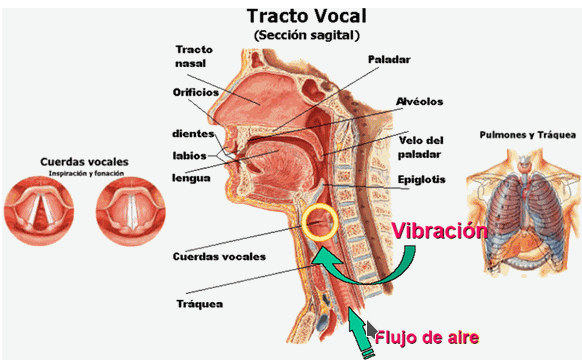
\includegraphics[width=\textwidth]{imagenes/03_02_aparato_fonador.png}
\end{figure}

El Alfabeto Fonético Internacional o IPA por sus siglas en inglés, fue estructurado desde 1888 y representa todas las posibles configuraciones para los fonemas que pueden ser ejecutados por el ser humano y la caracterización e identificación que da a las vocales es la que se puede observar en la tabla \ref{tab:ipa_table_vowels}


% \begin{landscape}
\begin{table}
\centering
\caption{Alfabeto Fonético Internacional: Vocales}
\label{tab:ipa_table_vowels}
\begin{tabular}{|l|l|l|l|l|l|l|}
\hline
{} & \multicolumn{2}{|c|}{Frontal} & \multicolumn{2}{|c|}{Central} & \multicolumn{2}{|c|}{Posterior}   \\
\hline
Cerrada & i  & y &\textbaru   & \textbari & \textturnm &  u  \\
\hline
Casi cerrada & \textsci  & \textscy &  \multicolumn{2}{|c|}{} &  & \textupsilon  \\
\hline
Semicerrada & e  & \textipa{\o} &\textreve &  \textbaro & \textramshorns & o \\
\hline
Intermedia &  \multicolumn{2}{|c|}{} & \multicolumn{2}{|c|}{\textschwa} &  \multicolumn{2}{|c|}{} \\
\hline
Semiabierta &\textepsilon  & \textipa{\oe} & \textrevepsilon & \textcloserevepsilon  & \textturnv & \textopeno \\
\hline
Casi abierta & \multicolumn{2}{|c|}{\ae} &\multicolumn{2}{|c|}{\textturna} &  \multicolumn{2}{|c|}{}  \\
\hline
Abierta & a  & \textscoelig &  \multicolumn{2}{|c|}{}  &\textscripta & \textturnscripta \\
\hline
\end{tabular}
\end{table}
% \end{landscape}

Además de estas alteraciones principales en las perturbaciones del aire, existen otros sonidos que interrumpen el flujo de aire emitido por el diafragma. Estos sonidos son denominados consonantes y son clasificados por su lugar de articulación y el tipo de articulación. El IPA también define una clasificación para las consonantes, la cual puede observarse en la tabla \ref{tab:ipa_table_pulmonic_consonants} y la tabla \ref{tab:ipa_table_non_pulmonic_consonants}

\begin{landscape}
\begin{table}
\centering
\caption{Alfabeto Fonético Internacional: Consonantes pulmónicas}
\label{tab:ipa_table_pulmonic_consonants}
\begin{tabular}{|p{25mm}|l|p{15mm}|l|l|p{15mm}|l|l|l|l|l|l|}
\hline
{} & Bilabial & Labio\newline dental & Dental & Alveolar & Post-\newline alveolar & Retrofleja & Palatal & Velar & Uvular & Faríngea & Glotal \\
\hline
Plosiva& p b  & & \multicolumn{3}{|c|}{t d} & \textipa{\:t \:d } & \textipa{c \*j} & k g &  q G & & \textipa{P} \\
\hline
Nasal& m &  \textipa{M} & \multicolumn{3}{|c|}{n} & \textipa{\:n}  &  \textipa{\*n}  & \textipa{N} & N &  & \\
\hline
Vibrante& B & & \multicolumn{3}{|c|}{r}  & & & & R &  & \\
\hline
Aproximante & & \textipa{v} & \multicolumn{3}{|c|}{\textipa{R}} & \textipa{\:r} & & & & &  \\
\hline
Fricativa  & \textipa{F B}& f v & \textipa{T D} & s z & \textipa{S z} & \textipa{\:s \:z} & \textipa{\c{c} J}& x \textipa{G} &\textipa{X  K}  &\textcrh \textipa{Q} & h\textipa{H}  \\
\hline
Lateral \newline fricative& & & \multicolumn{3}{|c|}{\textbeltl \textipa{\*z}} & & & & &  & \\
\hline
Aproximante & & \textipa{V}& \multicolumn{3}{|c|}{\textipa{\!R}} & \textipa{\:R} & j  & \textturnmrleg & & &  \\
\hline
Aproximante lateral& & \multicolumn{3}{|c|}{\textipa{l}} &  \textraisevibyi & \textturny & \textipa{\;L} & & & & \\
\hline
\end{tabular}
\end{table}
\end{landscape}

% \begin{landscape}
\begin{table}
\centering
\caption{Alfabeto Fonético Internacional: Consonantes no pulmónicas}
\label{tab:ipa_table_non_pulmonic_consonants}
\begin{tabular}{|p{20mm}|l|l|l|l|l|l|}
\hline
{} & Bilabial & Dental & Alveolar  & Palatal & Velar & Uvular   \\
\hline
Eyectiva \newline oclusiva& p\textipa{'}  & &t   & c\textipa{'} & k\textipa{'} &  q\textipa{'}  \\
\hline
Eyectiva \newline fricativa& \textipa{F'}  & \textipa{T'}&  s\textipa{'} & \textipa{\c{c}'} & x\textipa{'} & \textipa{X'}  \\
\hline
Click &\textipa{\!o}  & \textipa{|} & \textipa{!} &  & & \\
\hline
Implosiva & \textipa{\!b}  & \multicolumn{2}{|c|}{\textipa{\!d}} &  \textipa{\!j} & \textipa{\!g} & \textipa{\!G} \\
\hline
\end{tabular}
\end{table}
% \end{landscape}

El español utiliza solamente ciertos fonemas del IPA, y la representación de estos define los conocidos alfabetos fonéticos para el español. Entre los más conocidos se encuentran el SAMPA \cite{SAMPA}, y el Mexbet, el cual se representa en la tabla \ref{tab:mexbet} \cite{mexbet}.

\begin{table}[H]
\centering
\caption{Mexbet}
\label{tab:mexbet}
\begin{tabular}{|l|l|l|l|l|l|l|}
\hline
\textbf{Consonantes}         & \textbf{Labial}     & \textbf{Labio dental} & \textbf{Dental}     & \textbf{Alveolar}    & \textbf{Palatal}    & \textbf{Velar}  \\ \hline
Oclusivos Sordos             & p (p)&       & t (t)&       &       & k (k)\\ \hline
Oclusivos Sonoros            & b (b)&       & d (d)&       &       & g (g)\\ \hline
Africado Sordo               &      &       &      &       & tS (t\textipa{S}) &     \\ \hline
Fricativos Sordos            &      & f (f) &      & s (s) &       & x(x)\\ \hline
Fricativos Sonoros           &      &       &      &       & Z (\textipa{J})&     \\ \hline
Nasales                      & m (m)&       &      & n (n) & n$\sim$ (\textipa{\:n})             &     \\ \hline
Lateral                      &      &       &      & l (l) &                 & \\ \hline
Vibrante                     &      &       &      & r ({\textipa{\!R}})    &                 & \\ \hline
\end{tabular}
\end{table}

Para esto se realizó una anotación fonética manual sobre grabaciones del Open Speech Corpus \cite{Collazos2015} del subcorpus de palabras aisladas, el cual esta compuesto por 334 palabras distintas grabadas por múltiples locutores con un total de 9441 grabaciones de 39 locutores distintos, seleccionando aleatoriamente 100 palabras distintas y realizando una anotación manual por medio de PRAAT \cite{Praat}.

La anotación se realizo utilizando la convención definida en la tabla \ref{tab:anotacion_fonetica}. esta convención se uso considerando que el Open Speech corpus - words fue grabado en su totalidad por locutores latino americanos, del país Colombia y la región del Valle del Cauca. En esta representación fonética, se usa la palabra especial sil para determinar silencio; también se eliminan fonemas como la z fricativa dado que esta forma de pronunciación no es natural de la región de los hablantes.


\begin{table}[H]
\centering
\caption{Anotación Fonética}
\label{tab:anotacion_fonetica}
\begin{tabular}{|l|l|l|}
\textbf{Simbolo} & \textbf{Letra} & \textbf{Representación} \\ \hline
sil              & & Silencio                               \\ \hline
a                & a & vocal open central                   \\ \hline
b                & b &  consonante plosiva bilabial sonora   \\ \hline 
k                & c &  consonante plosiva palatal no sonora \\ \hline 
S                & ch &  consonante fricativa palatal        \\ \hline 
d                & d &  consonante plosiva dental sonora     \\ \hline 
e                & e &  vocal semi-open central              \\ \hline
f                & f &  consonante fricativa labiodental     \\ \hline 
g                & g &  consonante plosiva velar sonora      \\ \hline
i                & i &  vocal closed front                   \\ \hline
j                & j &  consonante approximant palatal       \\ \hline
l                & l &  consonante approximant alveolar      \\ \hline 
m                & m &  consonante nasal bilabial            \\ \hline 
n                & n &  consonante nasal alveolar            \\ \hline 
N                & ñ &  consonante nasal palatal             \\ \hline 
o                & o &  vocal semi-closed back               \\ \hline
p                & p &  consonante plosiva no sonora         \\ \hline 
R                & r &  consonante vibrant alveolar sonora   \\ \hline 
r                & r &  consonante vibrant alveolar no sonora \\ \hline
s                & s &  consonante fricativa alveolar         \\ \hline
t                & t &  consonante plosiva dental no sonora   \\ \hline
u                & u &  vocal closed back                    \\ \hline
y                & y &  consonante fricativa palatal         \\ \hline
\end{tabular}
\end{table}

La distribución de fonemas en la anotación manual se muestra en la tabla \ref{tab:distribucion_fonetica}

\begin{table}[H]
\centering
\caption{Distribución fonética}
\label{tab:distribucion_fonetica}
\begin{tabular}{|l|l|}
\textbf{Fonema} & \textbf{Ocurrencias} \\ \hline
sil & 173 \\ \hline
a   & 91  \\ \hline
o   & 79  \\ \hline
e   & 59  \\ \hline
n   & 45  \\ \hline
i   & 40  \\ \hline
l   & 31  \\ \hline
s   & 29  \\ \hline
t   & 27  \\ \hline
d   & 22  \\ \hline
R   & 22  \\ \hline
b   & 20  \\ \hline
r   & 19  \\ \hline
p   & 19  \\ \hline
j   & 16  \\ \hline
u   & 16  \\ \hline
m   & 15  \\ \hline
k   & 14  \\ \hline
g   & 11  \\ \hline
f   & 7   \\ \hline
c   & 5   \\ \hline
y   & 5   \\ \hline
C   & 2   \\ \hline
N   & 1   \\ \hline
S   & 1   \\ \hline
\end{tabular}
\end{table}

Las grabaciones seleccionadas se distribuyen entre 22 grabadas por locutores de género femenino, 68 masculinos y 10 no identificado.

En la imagen \ref{img:anotacion_fonetica_praat} se muestra la anotación fonética de realizada en Praat y en el archivo \ref{file:text_grid} el archivo correspondiente a la anotación fonética



\begin{figure}[H]
\caption{Anotación fonética con Praat}
\label{img:anotacion_fonetica_praat}
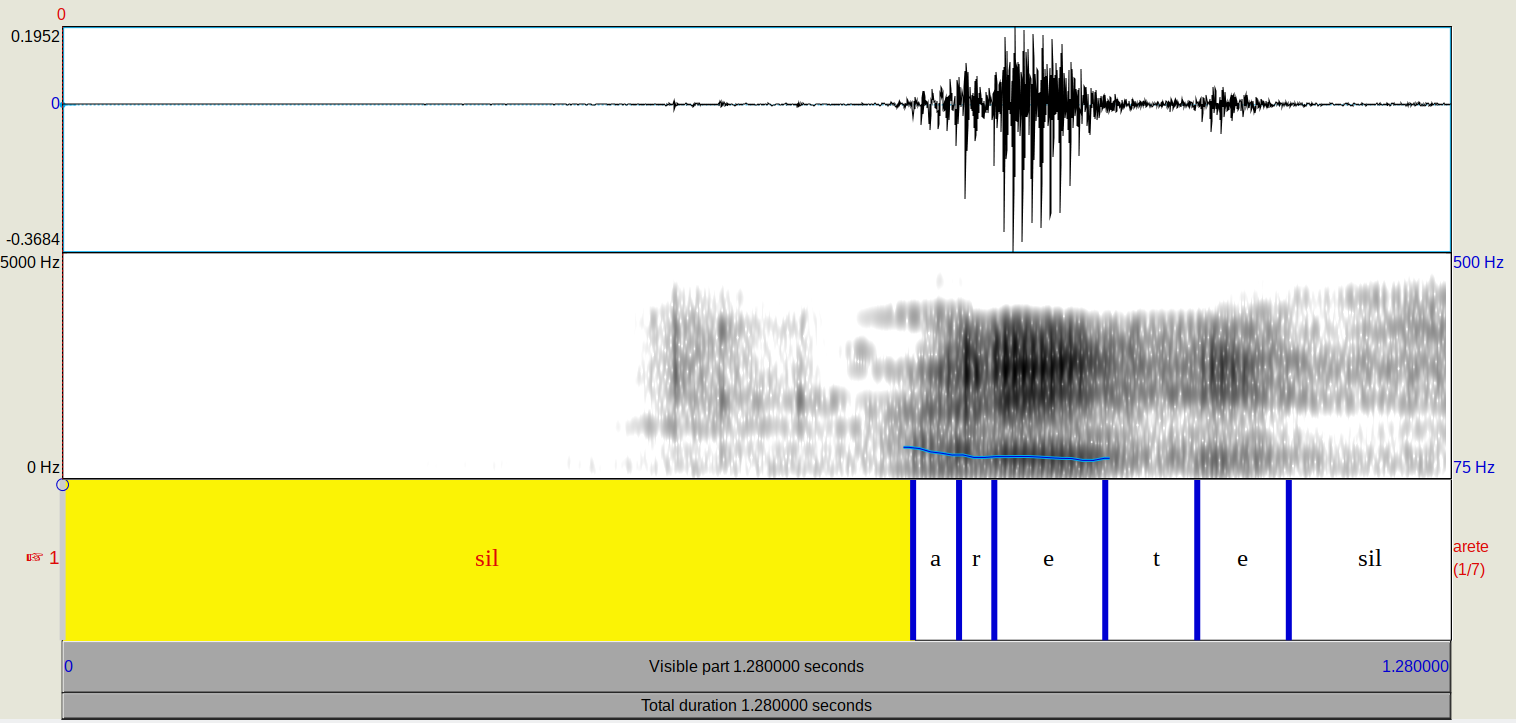
\includegraphics[width=\textwidth]{imagenes/03_01_anotacion_fonetica.png}
\end{figure}

\lstinputlisting[caption={Archivo TextGrid con anotación fonética}, label={file:text_grid}]{archivos/03_01_text_grid_ejemplo.txt}



\section{Anotación manual a nivel de sentencia}

También se realizó una anotación a nivel de declaración de los audiolibros de Librivox, seleccionando audios correspondientes a 6 horas de grabación, sobre los cuales se realizó una segmentación manual basada en símbolos de puntuación.

Para la selección de los audio libros, se ordenaron las grabaciones en orden ascendente considerando el tamaño del audio original en segundos, para posteriormente seleccionar 3 horas de locutores de género femenino y 3 horas del género masculino, garantizando de esta manera un balance de género y también la maximización de locutores diferentes. Cada archivo será identificado con un prefijo F o M que significa el género del locutor, separado por una línea baja \_ y el consecutivo asignado.

Los archivos almacenados en Librivox usan el formato de compresión con pérdida MP3, para su tratamiento son transformados a formato sin compresión WAV utilizando el programa Sox \cite{Sox}.

Se realizó de igual manera una descarga manual de los textos correspondientes a los audio libros seleccionados, generando archivos de texto plano cuya primera línea es el título del texto y el resto del archivo.

Como parte del pre-procesamiento del texto, se utilizaron expresiones regulares para segmentar los textos descargados de internet por símbolos de puntuación, y generando un nuevo archivo de texto plano donde cada línea contiene un índice, y la declaración correspondiente al segmento del texto.

Se muestra un ejemplo de texto tokenizado en el archivo \ref{file:texto_tokenizado}

\lstinputlisting[caption={Texto tokenizado}, label={file:texto_tokenizado}]{archivos/03_02_tokenizacion_texto.txt}

Los índices al comienzo de cada línea funcionan como identificadores en el proceso de anotación a nivel de declaración. Esto con el objetivo de facilitar el proceso de anotación al solo indicar en el campo de texto un índice en lugar del texto correspondiente. Posteriormente es posible reconstruir un archivo de anotación, reemplazando los índices por el texto correspondiente almacenado en el archivo de tokenización. El ejemplo de anotación de declaración del texto ejemplo se puede observar en el archivo \ref{file:text_grid_tokenizado}

\lstinputlisting[caption={Texto tokenizado}, label={file:text_grid_tokenizado}]{archivos/03_03_text_grid_tokenizado.txt}


\section{Anotación automática a nivel de sentencia usando Libri Vox Spanish}

\textcolor{red}{WIP}

Esta sección corresponde a la generación de TextGrids usando los archivos fuentes descargados directamente desde librivox y comparándolos con la segmentación manual de \cite{LibriVox-Spanish}, de momento no tengo nada acá mas que experimentos fallidos usando Onsets y de pronto luego miro si hay tiempo de dejar este capítulo si encuentro alguna luz. De pronto usando DTW pasa algo acá pero no se.


\chapter{Segmentación y Alineación automática}

Como la creación de recursos de manera manual es costosa, y los requerimientos de volúmen de información son altos, la generación automática o semi automática de recursos de habla toma gran relevancia en la investigación actual.

Dado que existen recursos abiertos y disponibles, pero no aptos para la invetigación, el procesamiento de estos de manera automática o semi automática debe garantizar nuevos recursos aptos para la investigación. Las tareas relacionadas con este problema son las de segmentación, la cual toma una señal de audio y extrae segmentos relevantes dentro de esta; la anotación, que toma una señal e identifica componentes de lenguaje dentro de esta y la alineación, que toma una señal e indica los lugares exactos en los cuales existe información de lenguaje.

El problema de la segmentación puede abordarse a nivel de declaración, palabra o fonema, y se presentan dos aproximaciones para realizar segmentación de audios.

\section{Segmentación basada en silencio}

Las segmentación basada en silencio es una respuesta natural al problema de como segmentar señales de voz, pues existe una correspondencia directa entre símbolos de puntuación y pausas en la voz. De igual manera en una señal de voz, los locutores requieren pausas para tomar aire, lo que permite que exista una cadencia en la señal y espacios donde realizar los cortes.

Para identificar el proceso de segmentación por silencios, es necesario entender como se almacenan las señales de voz digitalmente y como se puede procesar este tipo de datos.

La manera mas sencilla de representar digitalmente una señal de voz es haciendo el uso de la Modulación por Impulsos Codificados o PCM por sus siglas en inglés, donde por medio de un transductor análogo, se capturan las variaciones en la presión del aire y se registran como un rango de valores normalizado. El senso de la señal se hace periódicamente a una frecuencia determinada generando de esta manera una secuencia de valores que representa la señal. El proceso de representar la presión del aire en un segmento de tiempo se denomina cuantización, y para señales de audio se utilizan valores normalizados entre -127 y 128 a 16000 Hz de frecuencia.

En al figura \ref{img:pcm} se muestra la visualización de una grabación correspondiente a la palabra agua, en su longitud original y aumentada en un 500\% y 1000\% usando Audacity \cite{audacity}
\begin{figure}[H]
\caption{Representación visual de una señal de voz \cite{hableomsDeVoz}}
\label{img:pcm}
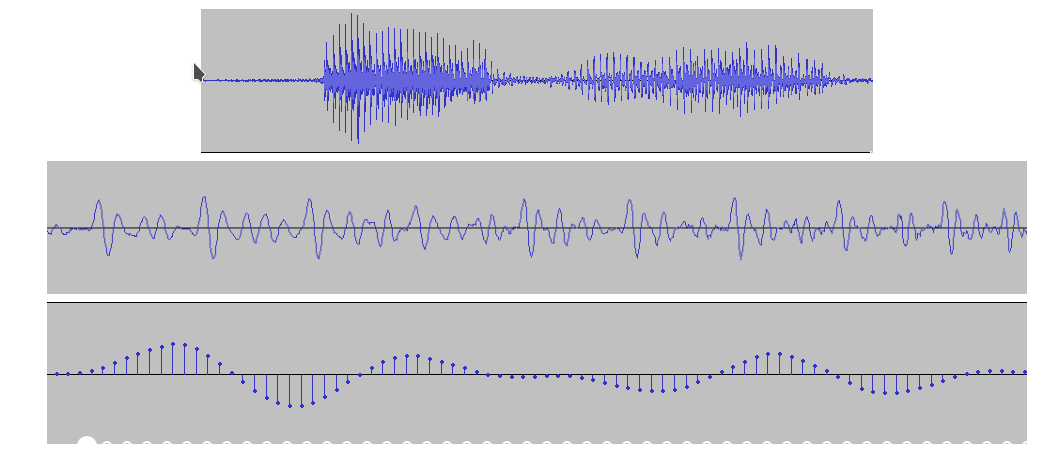
\includegraphics[width=\textwidth]{imagenes/04_01_pcm.png}
\end{figure}

Al hablar de silencio, nos referimos a ausencia total o parcial de sonido, lo cual se puede relacionar directamente con la intensidad de la señal en un segmento de tiempo.

Definiremos intensidad como la sumatoria de las energías en un periodo de tiempo  \cite{Jurafsky2000SpeechRecognition}    

\begin{equation}
\label{eq:energy}
I = \sum{x^2}  
\end{equation}

Esto nos daría un indicador de la toda la señal, sin embargo, es útil realizar este análisis por pequeños segmentos del audio para identificar en conjunto cuales son los puntos donde la intensidad baja representa un espacio de silencio. Estos segmentos por lo general se definen en espacios de 250ms solapados cada 100ms, aunque este solapamiento no es necesario para el proceso de identificación de intensidad, da la idea de que la señal es continua y que cada segmento comparte información con el anterior.

Utilizando esta idea es posible tomar cualquier señal de voz, segmentarla cada 250ms y encontrar los segmentos consecutivos donde la intensidad sea baja o cercana a cero y estos segmentos consecutivos representarían pausas de silencio.

Algunas consideraciones a tomar al usar esta aproximación es que incluso en medio de las señales de voz, existen subsegmentos donde la intensidad es baja, por ejemplo en la pronunciación de consonantes plosivas, como la b, c, d, g, p y t existe una interrupción momentánea y completa del flujo de aire, causando momentáneamente segmentos de silencio.

Usando las anotaciones fonéticas se determinó que la duración promedio de cada consonante plosiva es inferior a los 100ms, también realizando una anotación manual de sonidos y silencios sobre múltiples grabaciones de la anotación por declaración se determinó que los espacios de silencio entre frases eran de mínimo 500ms. De esta manera, utilizando segmentación de 250ms de longitud y desplazamiento de 100ms, se determinan como silencios los conjuntos de segmentos consecutivos de tamaño superior a cinco. 

Entendiendo la condición necesaria para determinar los silencios en una grabación de voz, es posible ejecutar el proceso asumiendo el silencio como ausencia completa de señal, sin embargo, salvo en condiciones muy especiales, donde exista un ambiente libre de ruido, como en un estudio de grabación con filtros físicos, análogos o digitales, en los espacios de silencio la intensidad no es estrictamente cero.

Mas aún, dependiendo de las condiciones y ambiente de grabación, los valores de intensidad en segmentos de silencio varían.

Considerando esto, se propusieron dos aproximaciones para determinar los segmentos de silencio, la primera normalizando los valores de la señal y definiendo un umbral fijo de intensidad en proporción al valor mas alto de la grabación, considerando valores de 0.3, 0.15 y 0.15 que representan umbrales de intensidad del 30\%, 15\%, y 5\%. También se experimentó utilizando algoritmos de agrupamiento con dos centroides iniciales en 0 y la intensidad máxima.

Los resultados se presentan en la tabla \ref{tab:resultados_segmentacion_silencios}

\begin{table}[H]
\centering
\caption{Resultados de la segmentación por silencios}
% \caption{Speech English Corpus}
\label{tab:resultados_segmentacion_silencios}
\begin{tabular}{|l|l|}
\hline
\textbf{Umbral} & \textbf{Precisión}  \\ \hline
Fijo 30\%       & 57.01\%             \\  \hline
Fija 15\%       & 83.26\%             \\  \hline
Fija 5\%        & 69.05\%             \\  \hline
Dinámico        & 74.53\%             \\  \hline
\end{tabular}
\end{table}


\section{Alineación basada en duración de fonemas}

\textcolor{red}{WIP}

Utilizando la segmentación basada en silencios, para determinar cuales son los textos correspondientes se realiza una alineación basada en la duración estimada de un segmento de texto y la duración de los segmentos calculados. Para esto se tomó la anotación fonética para determinar la duración promedio y la desviación estándar de la duración de cada fonema.

Dicha información se puede ver en la tabla \ref{tab:duracion_promedio_fonemas}

\begin{table}[H]
\centering
\caption{Distribución fonética}
\label{tab:duracion_promedio_fonemas}
\begin{tabular}{|l|l|l|}
\textbf{Fonema} &\multicolumn{1}{|p{2cm}|}{\textbf{Duración promedio}} & \multicolumn{1}{|p{2cm}|}{\textbf{Desviación estándar}} \\ \hline
sil & 0.6619 & 0.3700 \\ \hline
a   & 0.1421 & 0.0566 \\ \hline
o   & 0.1487 & 0.0607 \\ \hline
e   & 0.1204 & 0.0416 \\ \hline
n   & 0.1090 & 0.0442 \\ \hline
i   & 0.1294 & 0.0404 \\ \hline
l   & 0.1125 & 0.0530 \\ \hline
s   & 0.1811 & 0.1059 \\ \hline
t   & 0.0784 & 0.0507 \\ \hline
d   & 0.0877 & 0.0536 \\ \hline
R   & 0.0999 & 0.0517 \\ \hline
b   & 0.0826 & 0.0610 \\ \hline
r   & 0.0750 & 0.0254 \\ \hline
p   & 0.0692 & 0.0649 \\ \hline
j   & 0.1038 & 0.0659 \\ \hline
u   & 0.1441 & 0.0507 \\ \hline
m   & 0.1183 & 0.0515 \\ \hline
k   & 0.1224 & 0.0904 \\ \hline
g   & 0.1016 & 0.0970 \\ \hline
f   & 0.1402 & 0.0569  \\ \hline
c   & 0.1032 & 0.0838  \\ \hline
y   & 0.1118 & 0.0044  \\ \hline
C   & 0.1274 & 0.0248  \\ \hline
N   & 0.0575 & 0  \\ \hline
S   & 0.0927 & 0  \\ \hline
\end{tabular}
\end{table}

\section{Segmentación basada en información fonética de formantes en vocales}

\textcolor{red}{WIP}

La manera de entender los sonidos del lenguaje hablado ocurre por por la similaridad de los sonidos emitidos por cualquier locutor. Estas maneras de articular cada fonema permite que todos ellos tengan la misma una composición acústica similar.

Las vocales por ser sonidos de duración promedio mas alta y donde las características que las definen son pocas, unicamente la apertura de cuerdas bocales y la apertura de la boca, permiten que se caractericen utilizando una descomposición acústica.

Al descomponer cualquier señal utilizando la transformada de Fourier

\begin{equation}
\label{eq:fourier}    
f(x) = \frac{1}{2} \, a_{0} + \sum_{n=1}^{\infty} \left[
   a_{n}\,\boldsymbol{\cos} (n\,x) + b_{n} \,\boldsymbol{\sin} (n\,x) \right]
\end{equation}

Se obtienen señales raiz de cada onda compleja. Con las señales de voz, los coeficientes máximos  en el orden ascendente de la frecuencia se denominan formantes, y el formante 1 f1 y el formante 2 f2 representan efectivamente el fenómeno efectuado por las cuerda vocales vibrando y la resonancia dad por la cavidad bucal.

Para el idioma español los formantes teóricos par


\begin{table}[H]
\centering
\caption{Formantes teóricos para vocales del español.}
\label{tab:formantes_teoricos}
\begin{tabular}{|l|l|l|l|l|}
\hline
\textbf{Vocal} & \textbf{f1} & \textbf{f2} & \textbf{std f1} & \textbf{std f2} \\ \hline
a   & 638 & 36 & 1353 & 84 \\ \hline
e   & 458 & 42 & 1800 & 131 \\ \hline
i   & 286 & 6  & 2200 & 131 \\ \hline
o   & 460 & 19 & 1019 & 99 \\ \hline
u   & 300 & 20 & 992  & 121 \\ \hline

\end{tabular}
\end{table}

\begin{table}[H]
\centering
\caption{Formantes teóricos para vocales del español}
\label{tab:formantes_observador}
\begin{tabular}{|l|l|l|l|l|}
\hline
\textbf{Vocal} & \textbf{f1} & \textbf{f2} & \textbf{std f1} & \textbf{std f2} \\ \hline
a   & 682.84 & 1347.66 & 73.77 & 93.04 \\ \hline
e   & 494.84 & 1619.97 & 55.49 & 132.84\\ \hline
i   & 382.33 & 1657.33 & 50.65 & 155.24 \\ \hline
o   & 506.24 & 1101.14 & 60.20 & 170.64\\ \hline
u   & 434.77 & 984.185 & 50.32 & 193.66\\ \hline

\end{tabular}
\end{table}

Base teórica de los formantes 1 y 2 para vocales en español

Cálculo observado para formantes 

Gráfica de formante promedio +- desviación estandar sobre grabación vocálica

\addcontentsline{toc}{chapter}{Bibliography}
\bibliographystyle{plain}
% \bibliographystyle{apacite}
% \bibliography{bibliography/bibliography}
\bibliography{referencias_ante_proyecto.bib,custom_references_ante_proyecto.bib,references_chapter_1.bib}

\chapter{Conclusiones}

El presente trabajo exploró las tareas de segmentación y alineación del procesamiento de voz, reconociendo proponiendo aproximaciones computacionales apoyadas en el procesamiento digital de señales, la fonología y las ciencias de la computación para su resolución.

En los últimos tres años el incremento de recursos de licencia abierta en español para el procesamiento de voz ha aumentado considerablemente, mostrando la relevancia de estos recursos en la investigación.

Aproximaciones automáticas y colaborativas se han propuesto con éxito para la creación de recursos de voz.

Fuentes de datos de voz abiertas, como audio libros y grabaciones de sesiones parlamentarias, han sido usadas para la creación de corpus de voz.



\addcontentsline{toc}{chapter}{Bibliografía}
\bibliographystyle{apalike}
% \setcitestyle{authoryear,open={((},close={))}}
% \bibliographystyle{apalike}
% \bibliographystyle{apacite}
% \bibliography{bibliography/bibliography}
\bibliography{custom_references.bib,references.bib}



\end{document}
